\section{Aufbau und Durchführung}
\label{sec:Durchführung}
Im ersten Teil der Messung wird zwecks Untersuchung der 
Temperaturabhängigkeit des Sättigungsstroms bei fünf verschiedene
Heizleistungen jeweils die Diodenspannung kleinschrittig erhöht
und die Stromstärke der emittierten Elektronen abgelesen.\\
Es wird die Schaltung in \autoref{fig:temperatur} verwendet.\\

\begin{figure}[h]
    \centering
    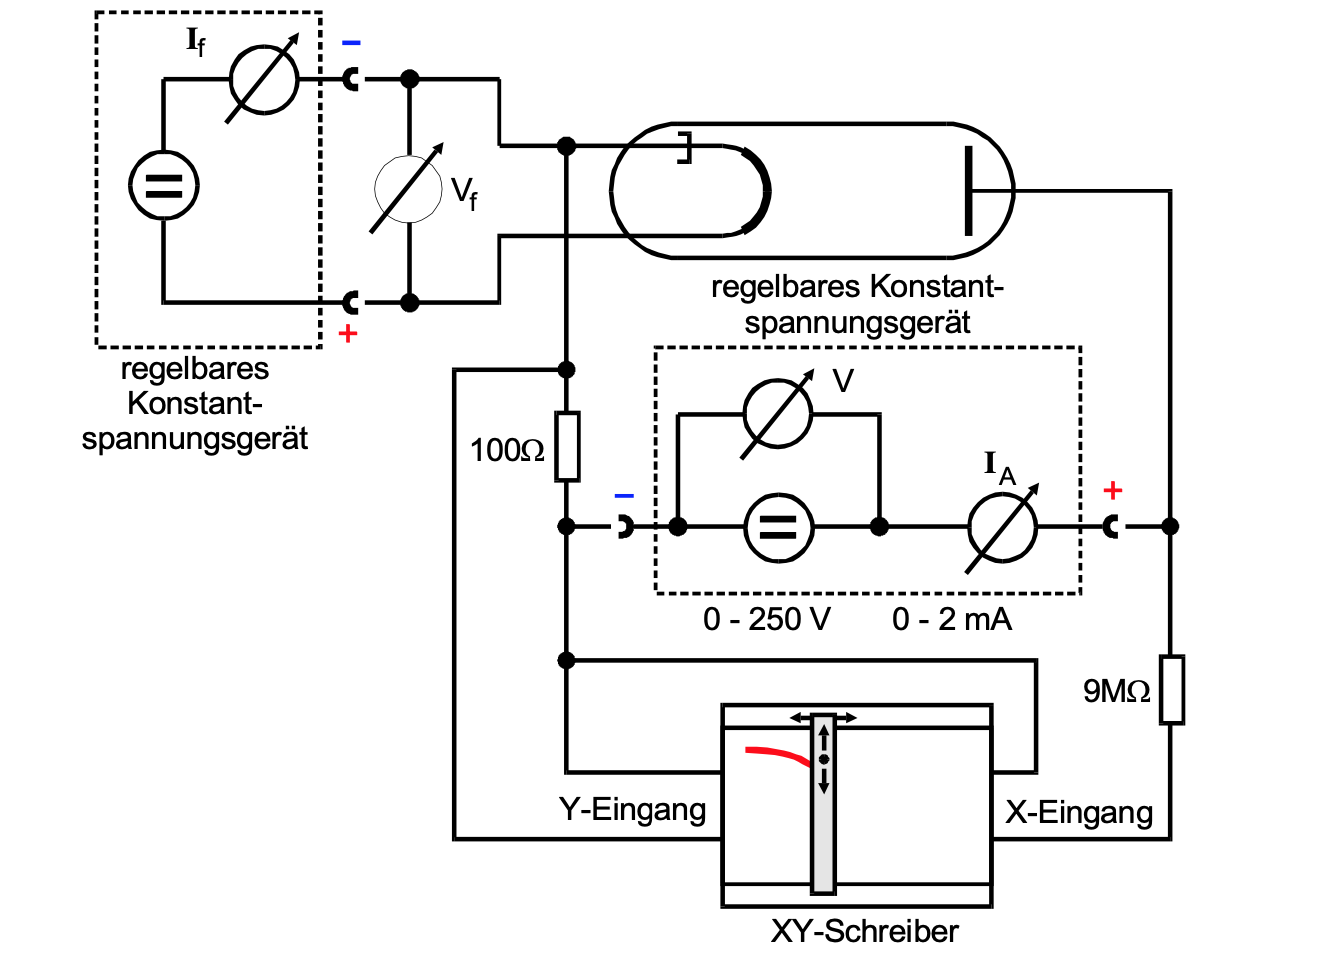
\includegraphics[width=\textwidth]{content/Aufbau1}
    \caption{Ersatzschaltbild des Aufbaus zur Bestimmung der Temperaturabhängigkeit.\cite{sample}}
    \label{fig:temperatur}
\end{figure}

Im zweiten Teil, zur Untersuchung der Anlaufstromkurve wird die folgende Schaltung 
\begin{figure}[h]
    \centering
    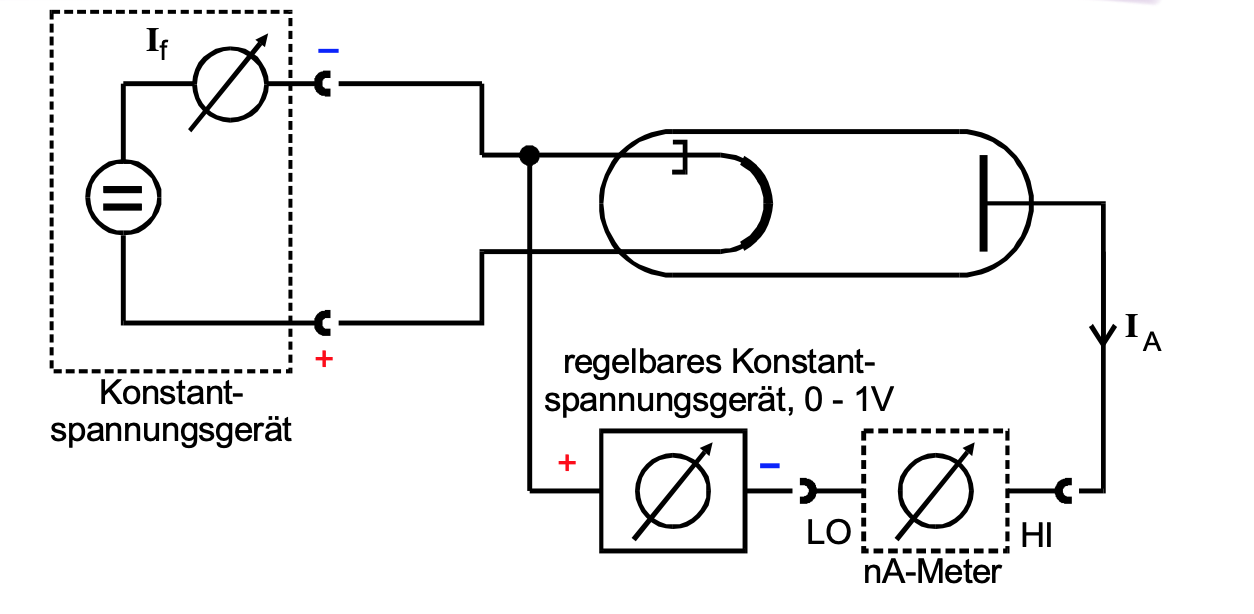
\includegraphics[width=\textwidth]{content/Aufbau2}
    \caption{Ersatzschaltbild des Aufbaus zur Untersuchung der Anlaufstromkurve.\cite{sample}}
    \label{fig:anlauf}
\end{figure}
verwendet. \\
Es wird bei maximaler Heizleistung die Anodenspannung kleinschrittig
erhöht und der Anodenstrom notiert. \\
